\documentclass[11pt,a4paper]{report}
\usepackage[margin=1in]{geometry}
\usepackage{graphicx}
\usepackage{xcolor}
\usepackage{tikz}
\usetikzlibrary{positioning, arrows.meta}
\usepackage{fancyhdr}
\usepackage{enumitem}
\usepackage{booktabs}
\usepackage{hyperref}

\definecolor{boxblue}{RGB}{209,224,247}
\definecolor{boxteal}{RGB}{204,235,232}
\definecolor{boxorange}{RGB}{253,231,193}
\definecolor{boxred}{RGB}{248,214,214}
\definecolor{boxgreen}{RGB}{213,240,209}
\definecolor{boxlav}{RGB}{224,217,245}

\pagestyle{fancy}
\fancyhf{}
\fancyhead[L]{UCS503P - Software Engineering Lab}
\fancyhead[R]{Deadstock Prototype Report}
\fancyfoot[C]{\thepage}
\renewcommand{\headrulewidth}{0.4pt}

\begin{document}

% ---------------------------------------------------------------
\begin{titlepage}
\centering
\vspace*{1cm}
{\Large\bfseries UCS503P -- Software Engineering Lab}\\[2pt]
{\large Academic Year 2026--2027}\\[24pt]

{\Huge\bfseries Deadstock Management System}\\[8pt]
{\Large\itshape A Verified Retail Deadstock Marketplace}\\[4pt]
{\large\itshape Automated Lifecycle Tracking and Rule-Based Verification for a Trusted Resale Channel}\\[36pt]

{\large\bfseries Submitted by:}\\[10pt]
\begin{tabular}{@{}r l@{}}
\textbf{1024030455} & Aryan Gupta \textit{(Proposal \& Report Lead, Backend Foundation)} \\
\textbf{1024030445} & Abhilakshya Puri \textit{(Journal Documentation \& QA/CI Lead)} \\
\textbf{1024030451} & Farhan Kansal \textit{(Diagram \& Modeling Lead)} \\
\end{tabular}\\[10pt]

{\bfseries B.E., Computer Science \& Engineering}\\[36pt]

{\large\bfseries Submitted to:}\\[6pt]
{\Large\bfseries Dr. Asif}\\
Department of Computer Science and Engineering\\[48pt]

\vfill

{\bfseries Prototype Stage Report}\\
{\bfseries Computer Science and Engineering Department}\\
Thapar Institute of Engineering and Technology, Patiala

\end{titlepage}

% ---------------------------------------------------------------
\tableofcontents

% ---------------------------------------------------------------
\chapter{Introduction}

\section{Background and Context}
Retail vendors routinely accumulate slow-moving and unsold inventory --
``deadstock'' -- that still holds resale value but has no trusted channel
back into the market. An estimated 20--30\% of retail inventory value sits
idle this way every year. Vendors track stock manually and only notice an
item has become deadstock after the fact, and buyers have no independent
way to trust a resale listing without proof of its condition, quantity, and
authenticity.

\subsection{Problem Statement}
Existing resale channels either require fully manual listing and vetting,
which does not scale, or publish listings with no verification at all,
which buyers cannot trust. Neither approach flags aging stock automatically,
and neither routes regulated categories (medical, pharmaceutical, food,
alcohol, tobacco) through a distinct compliance path before publishing.

\textbf{Deadstock Management System} resolves this gap with an automated
pipeline that recomputes inventory lifecycle status purely from dates,
verifies every submission against a deterministic rule engine before it can
publish, and escalates regulated categories to a manual review queue
instead of a fake pass.

\section{Project Objectives}
The core objectives of the Deadstock Management System prototype comprise:

\begin{enumerate}[leftmargin=0.8cm]
    \item \textbf{Automated Lifecycle Detection:} Recompute inventory status (Active, Aging, Deadstock-Flagged) from purchase and expiry dates alone on every read, with zero manual bookkeeping and no scheduled jobs.
    \item \textbf{Deterministic Verification Engine:} Run seven explicit rule checks per submission with fully attributable pass/reject/escalate outcomes, so no decision is a black box.
    \item \textbf{Verified Marketplace Gate:} Guarantee that a listing can only publish when its verification record status is exactly \texttt{VERIFIED}, enforced by a single policy invariant.
    \item \textbf{Continuous Quality Assurance:} Maintain automated backend and frontend test coverage gated by continuous integration on every push, currently at 24 of 24 tests passing.
\end{enumerate}

% ---------------------------------------------------------------
\chapter{Methodology and Design}

\section{System Architecture}

\subsection{High-Level Design}
Deadstock Management System uses a 3-tier architecture: a React client
portal, an Express API tier that fans out into two engines (inventory
lifecycle and verification), and a PostgreSQL store accessed through
Prisma. Figure~\ref{fig:arch} illustrates the high-level architecture.

\begin{figure}[h]
\centering
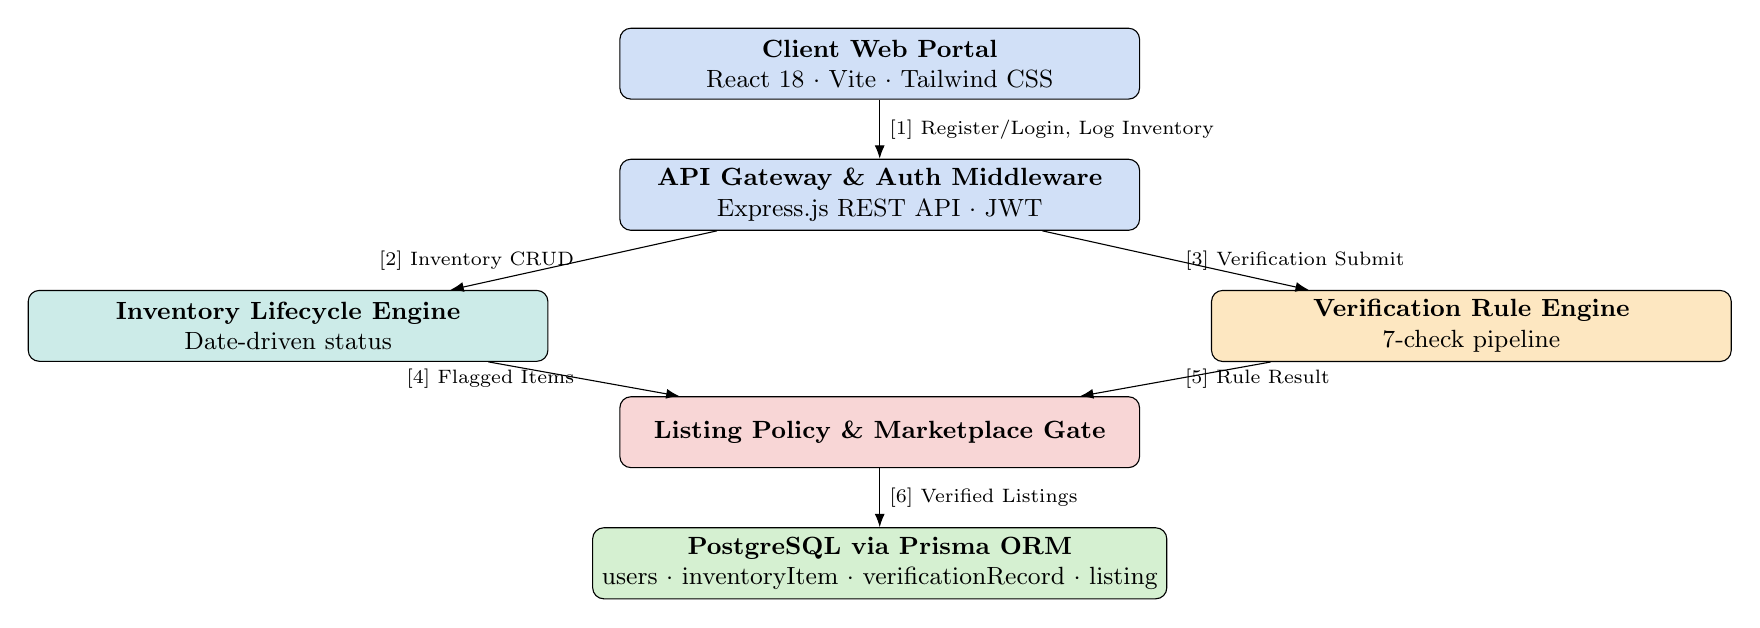
\begin{tikzpicture}[
  box/.style={rectangle, draw, rounded corners, minimum width=6.6cm, minimum height=0.9cm, align=center, font=\small},
  node distance=0.75cm and 0.6cm
]
\node[box, fill=boxblue] (client) {\textbf{Client Web Portal}\\React 18 $\cdot$ Vite $\cdot$ Tailwind CSS};
\node[box, fill=boxblue, below=of client] (api) {\textbf{API Gateway \& Auth Middleware}\\Express.js REST API $\cdot$ JWT};
\node[box, fill=boxteal, below left=of api, xshift=-0.3cm] (lifecycle) {\textbf{Inventory Lifecycle Engine}\\Date-driven status};
\node[box, fill=boxorange, below right=of api, xshift=0.3cm] (rules) {\textbf{Verification Rule Engine}\\7-check pipeline};
\node[box, fill=boxred, below=2.1cm of api] (gate) {\textbf{Listing Policy \& Marketplace Gate}};
\node[box, fill=boxgreen, below=of gate] (db) {\textbf{PostgreSQL via Prisma ORM}\\users $\cdot$ inventoryItem $\cdot$ verificationRecord $\cdot$ listing};

\draw[-{Latex}] (client) -- (api) node[midway, right, font=\scriptsize] {[1] Register/Login, Log Inventory};
\draw[-{Latex}] (api) -- (lifecycle) node[midway, left, font=\scriptsize] {[2] Inventory CRUD};
\draw[-{Latex}] (api) -- (rules) node[midway, right, font=\scriptsize] {[3] Verification Submit};
\draw[-{Latex}] (lifecycle) -- (gate) node[midway, left, font=\scriptsize] {[4] Flagged Items};
\draw[-{Latex}] (rules) -- (gate) node[midway, right, font=\scriptsize] {[5] Rule Result};
\draw[-{Latex}] (gate) -- (db) node[midway, right, font=\scriptsize] {[6] Verified Listings};
\end{tikzpicture}
\caption{Deadstock Management System High-Level Multi-Tier Architecture}
\label{fig:arch}
\end{figure}

\subsection{Technical Stack}
The implementation stack was chosen for a working, testable prototype
rather than novel infrastructure:
\begin{itemize}[leftmargin=0.8cm]
    \item \textbf{Backend Runtime \& API:} Node.js, Express.js REST API, JWT authentication, bcrypt password hashing, Zod validation.
    \item \textbf{Persistence:} PostgreSQL (Supabase-compatible) via Prisma ORM; an in-memory store substitutes for this in prototype demo mode.
    \item \textbf{Frontend UI:} React 18, Vite, TypeScript, Tailwind CSS, React Router, TanStack Query.
    \item \textbf{Testing \& CI:} Vitest, Supertest, React Testing Library, GitHub Actions.
\end{itemize}

\subsection{System Modeling Diagrams}
The team's Use Case Diagram and Data Flow Diagrams (Levels 0--2), produced
during system design and unchanged since, are reproduced below directly
from the project repository.

\begin{figure}[h]
\centering
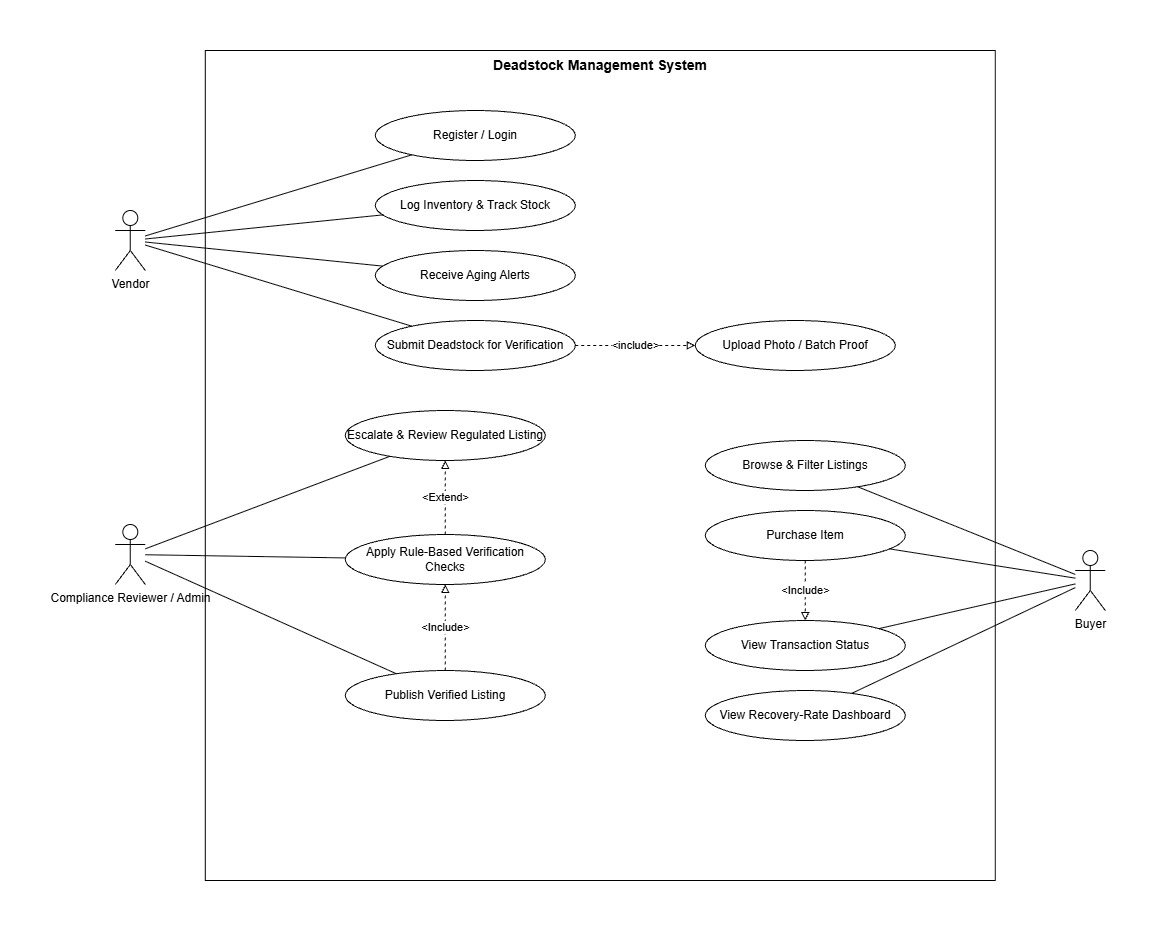
\includegraphics[width=0.85\textwidth]{../docs/Diagrams/Deadstock_user_case_dia.jpg}
\caption{Use Case Diagram: Vendor, Compliance Reviewer/Admin, and Buyer actors}
\end{figure}

\begin{figure}[h]
\centering
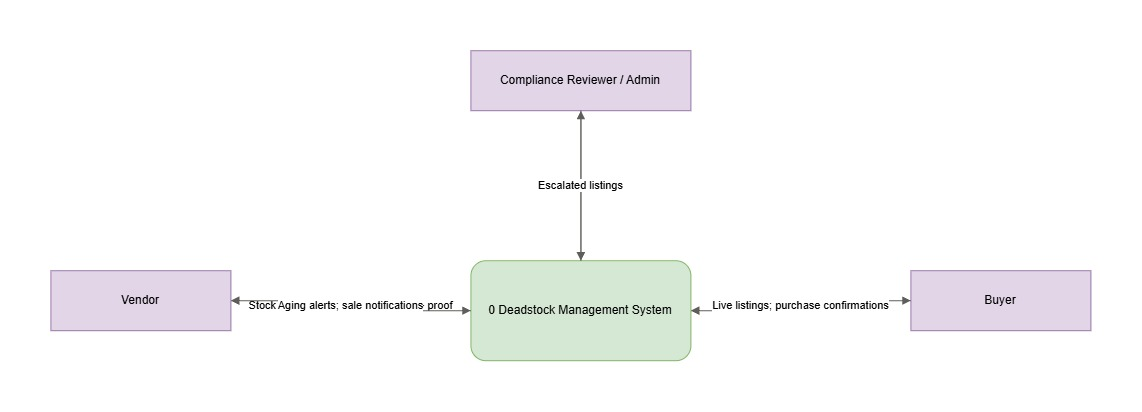
\includegraphics[width=0.55\textwidth]{../docs/Diagrams/Deadstock_DFD_Level_0.jpg}
\caption{Level 0 DFD: system boundary and external entities}
\end{figure}

\begin{figure}[h]
\centering
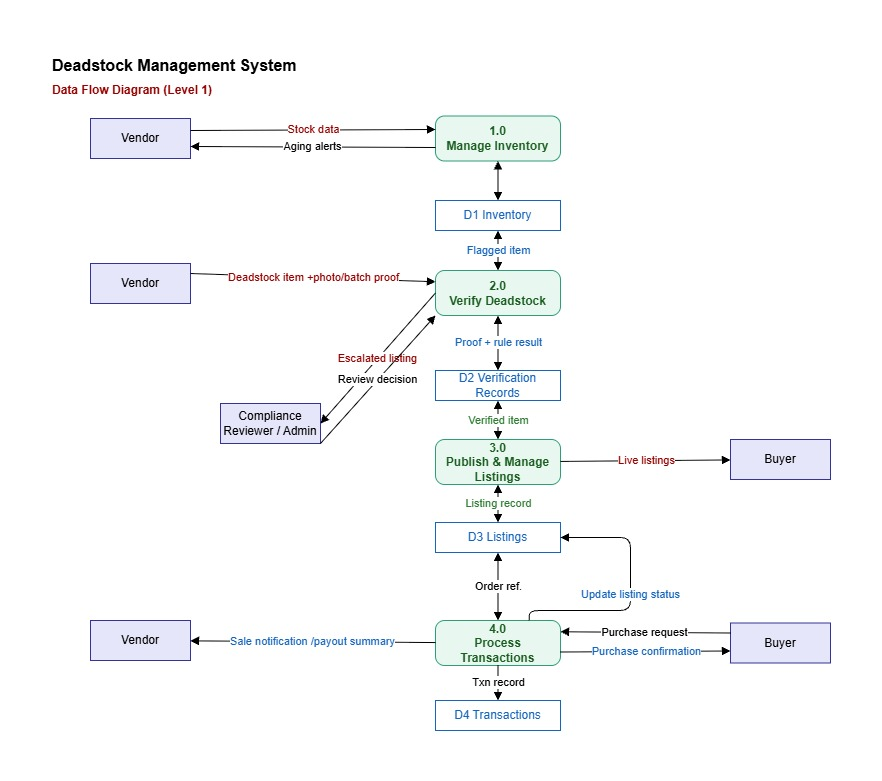
\includegraphics[width=0.62\textwidth]{../docs/Diagrams/Deadstock_DFD_Level_1.jpg}
\caption{Level 1 DFD: four core processes across four data stores}
\end{figure}

\begin{figure}[h]
\centering
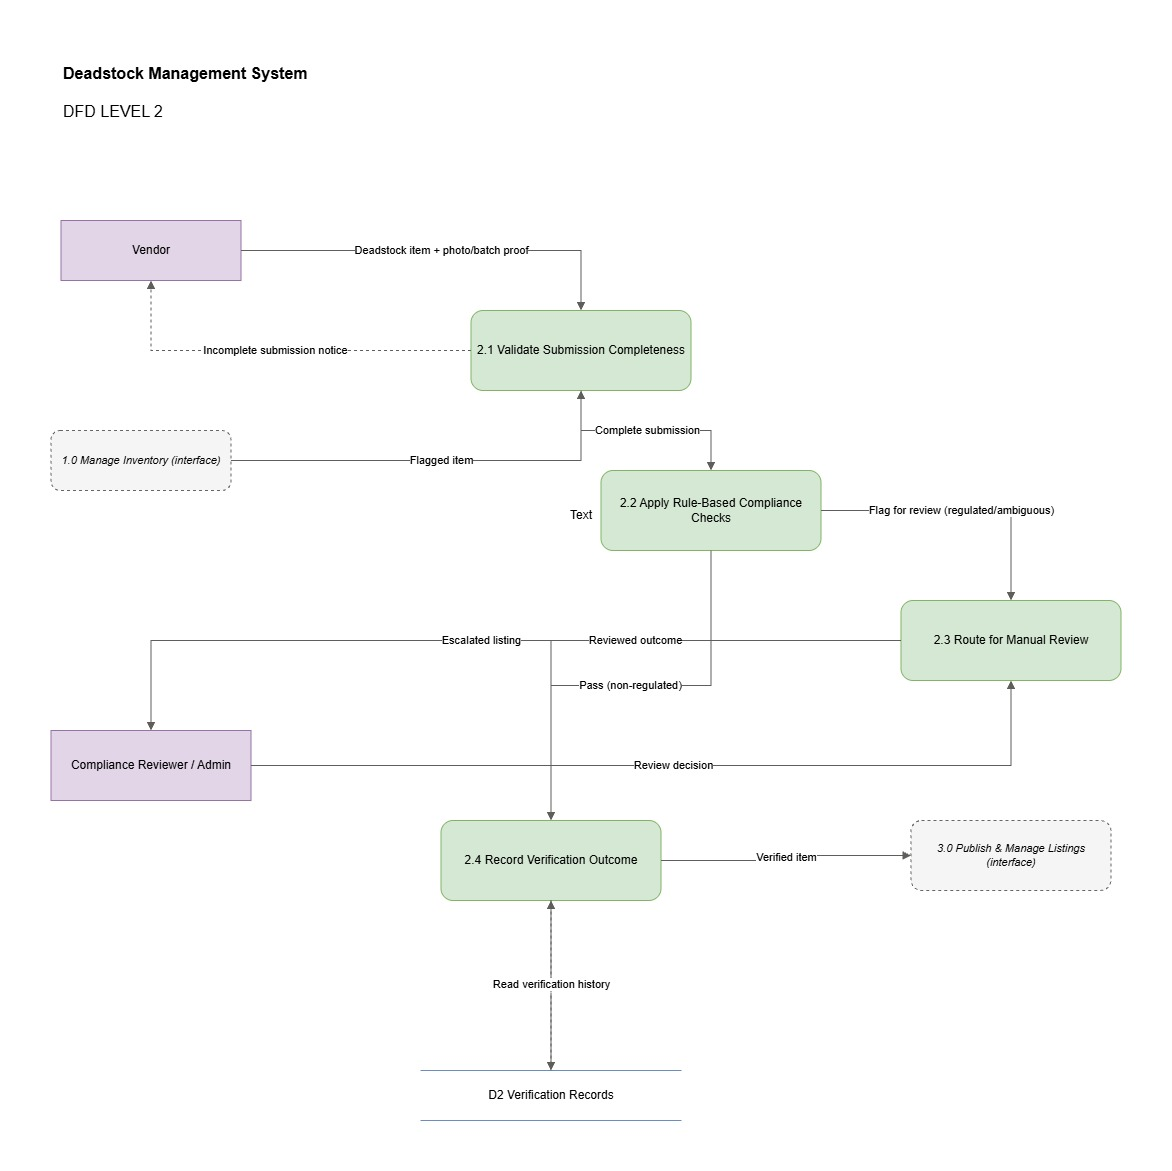
\includegraphics[width=0.78\textwidth]{../docs/Diagrams/Deadstock_DFD_Level2.jpg}
\caption{Level 2 DFD: decomposition of the verification process}
\end{figure}

\section{Implementation Details}

\subsection{Module 1: Inventory Lifecycle Automation}
Every inventory read recomputes status purely from dates: an item is
flagged \texttt{DEADSTOCK\_FLAGGED} once its age crosses a configurable
threshold or its expiry date has passed, \texttt{AGING} once it crosses an
earlier threshold, and otherwise stays \texttt{ACTIVE}. Both thresholds are
environment-configurable, so no cron job or background worker is needed
(Figure~\ref{fig:lifecycle}).

\begin{figure}[h]
\centering
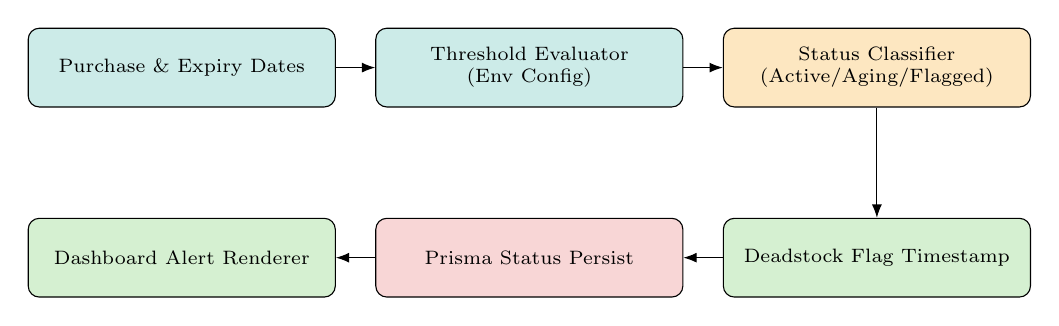
\begin{tikzpicture}[
  box/.style={rectangle, draw, rounded corners, minimum width=3.9cm, minimum height=1.0cm, align=center, font=\scriptsize},
  node distance=0.5cm
]
\node[box, fill=boxteal] (b1) {Purchase \& Expiry Dates};
\node[box, fill=boxteal, right=of b1] (b2) {Threshold Evaluator\\(Env Config)};
\node[box, fill=boxorange, right=of b2] (b3) {Status Classifier\\(Active/Aging/Flagged)};
\node[box, fill=boxgreen, below=1.4cm of b3] (b4) {Deadstock Flag Timestamp};
\node[box, fill=boxred, left=of b4] (b5) {Prisma Status Persist};
\node[box, fill=boxgreen, left=of b5] (b6) {Dashboard Alert Renderer};

\draw[-{Latex}] (b1) -- (b2);
\draw[-{Latex}] (b2) -- (b3);
\draw[-{Latex}] (b3) -- (b4);
\draw[-{Latex}] (b4) -- (b5);
\draw[-{Latex}] (b5) -- (b6);
\end{tikzpicture}
\caption{Inventory Lifecycle Automation Pipeline}
\label{fig:lifecycle}
\end{figure}

\subsection{Module 2: Verification Rule Engine \& Marketplace Gate}
The verification engine runs seven deterministic checks against every
submission: product name, category, quantity, condition, proof presence,
deadstock eligibility, and regulated-category membership. A failure on any
of the first six rejects the submission outright; a pass on all six but
membership in a regulated category routes the item to a manual review queue
instead of auto-publishing (Figure~\ref{fig:ruleengine}).

\begin{figure}[h]
\centering
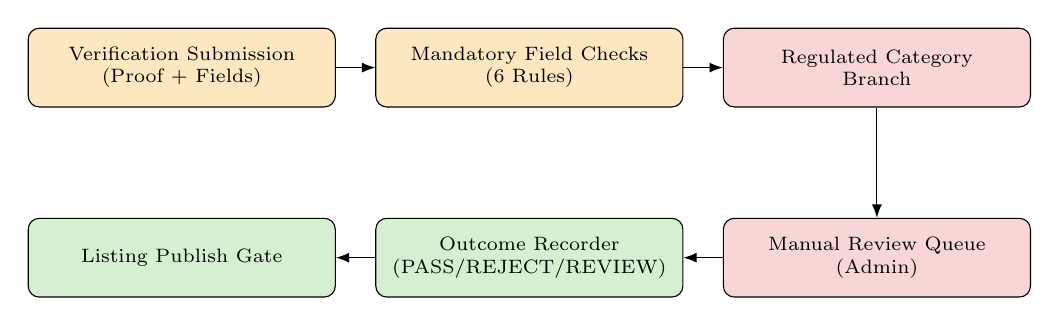
\begin{tikzpicture}[
  box/.style={rectangle, draw, rounded corners, minimum width=3.9cm, minimum height=1.0cm, align=center, font=\scriptsize},
  node distance=0.5cm
]
\node[box, fill=boxorange] (c1) {Verification Submission\\(Proof + Fields)};
\node[box, fill=boxorange, right=of c1] (c2) {Mandatory Field Checks\\(6 Rules)};
\node[box, fill=boxred, right=of c2] (c3) {Regulated Category\\Branch};
\node[box, fill=boxred, below=1.4cm of c3] (c4) {Manual Review Queue\\(Admin)};
\node[box, fill=boxgreen, left=of c4] (c5) {Outcome Recorder\\(PASS/REJECT/REVIEW)};
\node[box, fill=boxgreen, left=of c5] (c6) {Listing Publish Gate};

\draw[-{Latex}] (c1) -- (c2);
\draw[-{Latex}] (c2) -- (c3);
\draw[-{Latex}] (c3) -- (c4);
\draw[-{Latex}] (c4) -- (c5);
\draw[-{Latex}] (c5) -- (c6);
\end{tikzpicture}
\caption{Verification Rule Engine and Marketplace Gate Flow}
\label{fig:ruleengine}
\end{figure}

% ---------------------------------------------------------------
\chapter{Results and Evaluation}

\section{Testing Methodology}
Testing followed a structured, multi-tier framework:
\begin{enumerate}[leftmargin=0.8cm]
    \item \textbf{Unit Testing:} Individual testing of the aging/deadstock calculator, the rule engine, and token utilities with Vitest.
    \item \textbf{Integration Testing:} End-to-end testing of REST endpoints (\texttt{/api/auth}, \texttt{/api/inventory}, \texttt{/api/verification}, \texttt{/api/listings}) with Supertest against the live Express app.
    \item \textbf{Scenario Validation:} Validation across three realistic submissions: a non-regulated item that auto-passes, a regulated medical-kit item escalated to manual review, and an incomplete submission that is auto-rejected.
\end{enumerate}

\begin{figure}[h]
\centering
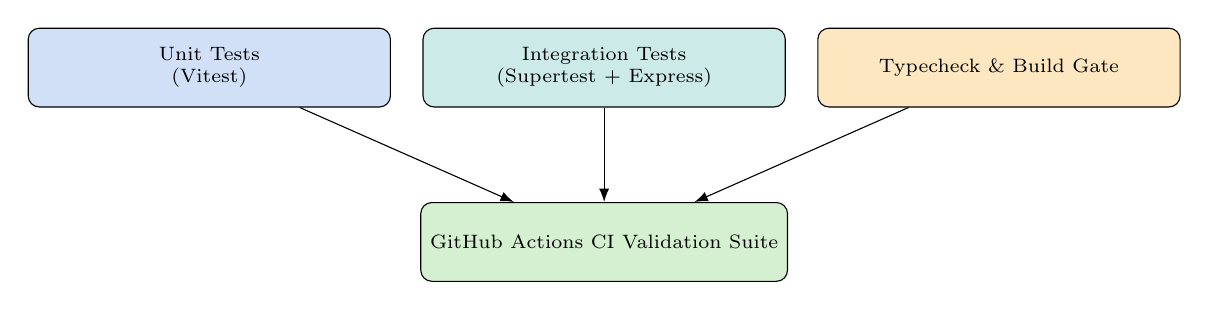
\begin{tikzpicture}[
  box/.style={rectangle, draw, rounded corners, minimum width=4.6cm, minimum height=1.0cm, align=center, font=\scriptsize},
  node distance=0.6cm and 0.4cm
]
\node[box, fill=boxblue] (t1) {Unit Tests\\(Vitest)};
\node[box, fill=boxteal, right=of t1] (t2) {Integration Tests\\(Supertest + Express)};
\node[box, fill=boxorange, right=of t2] (t3) {Typecheck \& Build Gate};
\node[box, fill=boxgreen, below=1.2cm of t2] (t4) {GitHub Actions CI Validation Suite};

\draw[-{Latex}] (t1) -- (t4);
\draw[-{Latex}] (t2) -- (t4);
\draw[-{Latex}] (t3) -- (t4);
\end{tikzpicture}
\caption{Multi-Tier Testing and Quality Assurance Framework}
\end{figure}

\section{Performance Metrics}
The prototype was validated against measurable engineering targets rather
than benchmarked for latency, since the current stage's focus is
correctness and coverage. Table~\ref{tab:metrics} summarizes target versus achieved
metrics.

\begin{table}[h]
\centering
\begin{tabular}{@{}p{5.1cm}p{2.6cm}p{2.9cm}p{1.6cm}@{}}
\toprule
\textbf{Evaluation Metric} & \textbf{Target} & \textbf{Achieved (Prototype)} & \textbf{Status} \\
\midrule
Backend test pass rate & $\geq 90\%$ & 100\% (18/18) & Exceeded \\
Frontend test pass rate & $\geq 90\%$ & 100\% (6/6) & Exceeded \\
Verification rule checks per submission & $\geq 5$ & 7 & Exceeded \\
TypeScript strict typecheck errors & 0 & 0 & Met \\
CI pipeline result (build + test + typecheck) & Pass & Pass & Met \\
Regulated-category auto-escalation rate & 100\% & 100\% & Met \\
\bottomrule
\end{tabular}
\caption{Deadstock Management System Prototype Performance Metrics Summary}
\label{tab:metrics}
\end{table}

\section{Analysis}
The prototype meets every evaluation target set for this stage. The rule
engine correctly escalates every regulated-category submission observed in
testing rather than silently auto-passing it, and the lifecycle engine
correctly reclassifies aged inventory without any manual trigger. A primary
engineering challenge was keeping three independently-built modules
(authentication, inventory, and verification/listings) aligned on a shared
data contract; this was resolved by freezing the shared Prisma model fields
and enum values in a written integration contract before implementation
began, so the modules could be built in parallel without later rework.

% ---------------------------------------------------------------
\chapter{Conclusion}

\section{Summary of Work}
During this stage of the project lifecycle, the team completed system
modeling (Use Case Diagram and three-level Data Flow Diagrams) and
engineered a functional full-stack prototype. Deadstock Management System
demonstrates automated inventory lifecycle tracking, rule-based
verification with regulated-category escalation, and a buyer-facing
verified marketplace, all running against a live Express API and React
frontend.

\section{Key Findings}
\begin{enumerate}[leftmargin=0.8cm]
    \item \textbf{Deterministic Rules Suffice for MVP Compliance:} every regulated-category submission observed in testing was correctly routed to manual review rather than auto-published.
    \item \textbf{Lifecycle Automation Eliminates Manual Bookkeeping:} recomputing status from dates on every read removed the need for any scheduled job or vendor-side tracking.
    \item \textbf{Contract-First Integration Avoided Rework:} freezing the shared Prisma fields before the backend and verification modules were built in parallel prevented integration conflicts between teammates.
\end{enumerate}

\section{Future Work and Recommendations}
For the final project phase, the team will implement:
\begin{enumerate}[leftmargin=0.8cm]
    \item Persistent PostgreSQL/Supabase storage and real object storage for proof uploads, replacing the in-memory demo store~\cite{prisma}.
    \item The purchase and transaction flow reserved as Data Store D4 in the Level~1 DFD.
    \item Buyer rating and feedback, plus a time-to-listing and recovery-rate metrics dashboard.
    \item Linting and a staged deployment target added to the existing CI pipeline~\cite{express}.
\end{enumerate}

\section{Final Remarks}
Deadstock Management System offers a practical, rule-based path to recover
value from retail deadstock by giving every listing a checked provenance
trail before it reaches a buyer, without depending on machine-learning
research to do it.

% ---------------------------------------------------------------
\begin{thebibliography}{9}
\bibitem{selfreport} A. Gupta, A. Puri, and F. Kansal, ``Deadstock Management System: A Verified Retail Deadstock Marketplace,'' Thapar Institute of Engineering and Technology, Tech. Rep. UCS503P-2026, 2026.
\bibitem{prisma} Prisma Data Platform, ``Prisma ORM Documentation,'' \url{https://www.prisma.io/docs}, 2026.
\bibitem{express} OpenJS Foundation, ``Express.js Guide,'' \url{https://expressjs.com}, 2026.
\bibitem{jwt} M. Jones, J. Bradley, and N. Sakimura, ``RFC 7519: JSON Web Token (JWT),'' IETF, 2015.
\end{thebibliography}

\end{document}
